\chapter{Deseño e implementación do dispositivo}
\label{chap:implementacion_dispositivo}
Neste capítulo afondarase no desenvolvemento do dispositivo comezando polo aspecto físico, opcións dispoñibles e alternativas, seguido pola construción do dispositivo e a implementación do sofware tendo en conta os problemas xurdidos e as solucións aplicadas.


\section{Esquema xeral do dispositivo HW}


As esixencias principais destes dispositivo son a existencia de conexións para as luces leds, conexións para unha cámara e capacidade de procesamento e comunicación o que engadiremos unha quinta esixencia, xa que o obxectivo do proxecto e conseguir unha solución de hardware e software libre que posibilite que o usuario final poida adquirir os compoñentes e montalos de forma sinxela, é preciso que os compoñentes sexan fáciles de adquirir e traballar con eles.

A continuación analizaranse as diferentes opción de hardware dispoñibles, as súas características e seus pros e contras para o proxecto proposto.

\subsection{Placas de desenvolvemento}


Sendo o desenvolvemento dunha placa dedicada a este propósito a solución idílica, o custo de este proceso xunto coa dificultade final da construción, sempre que non se optase por unha produción en serie, son as principais contras desta opción. Poren optarase por elixir unha placa cos requisitos requiridos entre as posibles opcións dispoñibles no mercado. Centrarémonos nos modelos co menor tamaño posible.

As placas contempladas son as seguintes:

\begin{itemize}
    \item Arduino

Arduino é unha compañía dedicada o deseño e produción de placas de desenvolvemento con software e hardware, o que permite que terceiras compañías produzan as súas placas permitindo prezos finais de produto moi baixos.

Con un ide propio cunha linguaxe de programación baseada en C++, cunha ampla compatibilidade con diverso hardware, a diversidade de opcións e a sua facilidade de uso converte as súas placas nas mais populares do mercado.

Polo seu tamaño e forma as placas Arduino consideradas son as seguintes:
    \begin{itemize}
        \item Arduino Micro e Arduino Nano

O primeiro esta baseado no microcontrolador de 8bits ATmega32U4 cunha frecuencia de 16MHz, 32KB de memoria flash e 2.5KB de \emph{SRAM}.
Conta con 20 pins de entradas/saídas dixitais con 7 canles \emph{PWM} e 12 pins de entradas analóxicas.

O segundo baséase no microcontrolador de 8bits ATmega328 traballando a unha frecuencia de 16MHz, conta con 32KB de memoria flash e 2KB de \emph{SRAM}. Conta con 22 pins de entradas/saídas dixitais dos cales 6 son \emph{PWM} tamén conta con 8 pins de entradas analóxicas.

Estas dúas versión o contar con gran cantidade de pins tanto dixitais como analóxicos e un consumo enerxético e moi baixo xunto cun baixo prezo inferior os 5 euros nas versións de fabricantes de terceiros fainos perfectos para o propósito de control de leds, pero a sua baixa potencia computacional dificultaría o procesamento de vídeo. Tampouco conta co hardware necesario para as comunicación sen fíos.

        \item Arduino MKR ZERO e Arduino MKR1000

Ambos baseado no procesador ARM M0+ de 32 bit de baixo consumo cunha frecuencia de funcionamento de 48MHz, 256KB de memoria flash e 32kB de \emph{SRAM}, contan con 7 entradas analóxicas e 1 saída analóxica e 12 pins poden funcionar como PWM. Inclúe conexións \emph{SPI} \emph{UART} e \emph{I2C}. Tamén inclúen unha conexión para alimentalos directamente cunha batería de 3.7v. A diferencia entre ambos e que o primeiro conta con 22 pins de entrada e saída dixital mentres que o segundo conta con 8 pero inclúe un chip Wi-Fi.

Ambos teñen as capacidades de procesamento necesarias para a xestión das luces, do vídeo e as conexións. O único punto negativo é que as cámaras compatibles a nivel de conexión e librerías con estas placas non dispoñen de moita calidade de vídeo.

Estas placas poden obterse por entre 20 e 50 euros

        \item Arduino MKR VIDOR 4000

Esta placa de desenvolvemento a parte do procesador ARM M0+ inclúe un chip \emph{FPGA} que permite a sua configuración como diferentes hardware permitido que a placa poda dispoñer de diferentes compoñentes configurables como podería ser múltiples USB ou chips aceleradores de vídeo. Aparte conta con conexión micro HDMI mini PCI Express e un conector de cámara \emph{MIPI} no que se poderían conectar diversas cámara con calidade mais que suficiente para este proxecto.

O seu prezo e superior os 60 euros.
    \end{itemize}
    \item Raspberry Pi

As Raspberry Pi son unha serie de placas de desenvolvemento cun prezo moi axustado e unha potencia suficiente para para pode executar un sistema operativo completo. Grazas a sua popularidade dispón dun amplo soporte e compatibilidade con diversos software e outras plataformas hardware que a fan perfecta para diversos proxectos, como robótica, \emph{IoT} ou centros multimedia.
A versión dispoñible con menor tamaño e a Raspberry Pi Zero
    \begin{itemize}
        \item Raspberry Pi Zero e Raspberry PI Zero W

Esta placa conta cun microprocesador baseado na arquitectura ARM de 32bits que funciona a 1GHz, acompañase de un procesador de vídeo e unha memoria ram de 512MB. No apartado de conexións conta con un micro USB de carga e outro de datos, unha saída de vídeo HDMI e outra analóxica, unha rañura para unha tarxeta micro sd e un conector de cámara CSI. Tamen conta con 20 pins de conexión que a dotan de entradas e saídas dixitais, dúas canles \emph{PWM}, conexiós \emph{SPI} \emph{I2C} e \emph{UART} xunto a conexións de 5v, 3.3v e terra. A versión Zero W tamén dispón dun chip Wi-Fi e Bluetooth.
A sua potencia e capacidade de conexión a fan máis que capaz de para este proxecto, e o seu prezo, 5 e 10 euros respectivamente, é unha das súas principais vantaxes.
    \end{itemize}
    \item ESP8266 e ESP32

A principal característica destas placas é que implementan chips Wi-Fi e Wi-Fi máis Bluetooth respectivamente,contan cun procesador \emph{RISC} de un ou dous núcleos con velocidades dispoñibles entre os 80MHz e 240MHz e memorias ram de entre 32KiB e 520KiB.

Os seus múltiples portos e interfaces,\emph{SPI} ,  \emph{I2C}, \emph{UART}, \emph{PWM} entre outros, o seu baixo consumo e a sua compatibilidade co entorno de programación de arduino fainos ideais para pequenos proxectos de \emph{IoT}, robótica ou domótica. Segundo as súas características poden obterse dende o prezo de un euro.

O igual que pasaba coas placas Arduino os ESP son ideais para a parte do manexo das luces pero non para a xestión do vídeo.
    \item Outras placas baseadas en procesadores ARM

NO mercado existen múltiples placas de desenvolvemento baseadas en procesadores ARM, non obstante o prezo e o soporte da Raspberry Pi faina a mellor opción para a maioría de proxectos mais xenéricos.
    \item Outras placas baseadas en \emph{FPGA}

Os chip \emph{FPGA} permiten un nivel de personalización hardware moi elevado, pero tamén contan cun alto prezo, e na maioría dos casos cun \emph{toolchain} privativo que e necesario pagar para poder desenvolver en eles. O contrapunto a sua versatilidade é un maior custo de desenvolvemento en comparación con solucións de programación de alto nivel.
\end{itemize}
Tendo en conta o tamaño, a potencia, as conexións dispoñibles e o prezo, decidiuse optar pola Raspberry Pi Zero e Zero W como a placa encargada do control das luces e do vídeo.

\subsection{Luces led}
As dúas principais vantaxes das luces led fronte a outras formas de iluminación son o se baixo consumo e o seu pequeno tamaño. Estas calidades fainas ideais para un dispositivo portátil coma o que pretendemos construír.
Os requirimentos principais son poder controlar a intensidade dos leds e dispoñer de polo menos un color vermello para indicar a posición e a freada, e un color amarelo ou ámbar para os intermitentes.

Coa intención de miniaturizar se optara por utilizar leds \emph{RGB} que permiten xerar diversas combinacións de cores e así poder utilizar os mesmos leds para as diferentes funcións.
Xa que a Raspberry Pi non conta con saídas analóxicas, utilizaranse as canles \emph{PWM} que permite enviar sinais moduladas en pulsos. A modulación \emph{PWM} permite acender e apagar os leds múltiples veces a unha alta frecuencia a unha velocidade, tan rápidas que o ollo humano percibe como diferentes intensidades lumínicas en función da anchura dos pulsos. En leds \emph{RGB} compatibles o \emph{PWM} tamén se pode utilizar para codificar a cor elixida, e en series de leds conectados e direccionables se pode elixir que led a iluminar e a súa cor e intensidade individualmente, permitindo así controlar un alto numero de leds cunha soa saída \emph{PWM}.

Existen diferentes tipos de leds \emph{RGB} direccionables no mercado, elixiremos o tipo de led en función do seu tipo de conexión, a dispoñibilidade de librerías de software compatibles e coa limitación de que deberán operar a 5v que a voltaxe constante que necesita a Raspberry Pi para funcionar.\\

Os tipos de led direccionables analizados son:
\begin{itemize}
    \item WS2812B e WS2813

Estes leds inclúen un circuíto integrado en cada led que o conectalos en serie permite o control dunha secuencia teoricamente infinita de leds. Cada led conta con tres entradas e tres saídas: voltaxe, terra e datos. A información a pasar os leds se formara cun fluxo de datos a almacenar nun \emph{buffer} en memoria, ocupando a información de cada un 3 bytes, e se pasarán o primeiro led que lerá os primeiros 24 bits coa información da intensidade de cada cor, vermella, verde e azul, e pasará o resto de datos o seguinte led.

Cada led tarda 30 microsegundos en recibir os datos e 50 microsegundos e actualizar a sua cor, o atraso de transmisión entre leds e de 0.5 microsegundos. O consumo máximo de cada led e de 60 mA a 5V.

Os WS2813 engaden unha segunda liña de datos para que se un led deixa de funcionar os seguintes poidan seguir recibindo a información.
    \item SK6812

Estes leds comparten a maioría de características dos WS2812B coa diferencia de que aumenta a sua taxa de refresco a 1.2KHz con respecto os 400Hz dos WS2812B. Tamén engaden unha cuarta cor branca en cada led.

O a nivel de software son compatibles con WS2812B pero as súas diferenzas non permiten a sua interconexión física.
    \item APA102 e APA102C

Estes leds contan cunha interface SPI que conta cunha sinal de datos é outra de reloxo. Isto e para solucionar o problema de sincronización que se poden producir cando os led son manexados dende placas con capacidade de multitarefa sen un \emph{kernel} especifico para entrada e saída a tempo real. Tamén aumenta sua taxa de refresco ata os 19.2kHz.
\end{itemize}

Sendo os leds APA102 superiores en características os outros dous, contan coa desvantaxe de que requiren máis cables de conexión. As súas vantaxes a nivel de velocidade e sincronismo son esencias para a xeración de imaxes ou vídeo pero non para simples animacións como as que utilizaremos neste proxecto. Porén optaremos por utilizar os leds WS2812B e WS2813 ou SK6812.

Este tipo de leds están dispoñibles en diferentes combinacións: leds individuais, tiras flexibles, tiras ríxidas, aneis e matrices. Faremos probas con tiras e aneis de diferentes tamaños.


\subsection{Cámara}

No caso da cámara plantexanse dúas opcións utilizar unha cámara usb ou unha das cámara deseñadas para funcionar coa Raspberry Pi que utilizan a sua conexión \emph{CSI}. Optaremos pola segunda opción xa que unha cámara usb implica un tamaño demasiado grande para o proxecto e ademais non soen estar indicadas para a iluminación de exteriores.

No mercado existen diversos módulos de cámara para a Raspberry Pi pero a maioría están baseados nos Raspberry Pi Camera Module V1 e Raspberry Pi Camera Module V2 a principal diferencia entre ambos e que o primeiro conto con 5 megapixeles mentres o segundo conta con 8 megapixeles e unha notable mellora na calidade de imaxe.\\

As principais diferenzas nos módulos dispoñibles no mercado son:
\begin{itemize}
    \item Tamaño

Existen versións especificas para a Raspberry Pi Zero máis pequenas pero solo do Camera Module V1, as versións normais xa contan cun tamaño moi axustado.

    \item Presenza de filtro infravermello

As cámara soen contar cun filtro de luz infravermella para evitar o \emph{aliassing} que se produce nas cámara xa que as pantallas que utilizamos non están destinadas para emitir infravermellos e os nosos ollos non son capaces de percibilos. As cámaras que non contan con este filtro dan como resultado imaxes mais luminosas e cunha tonalidade violácea. Estas cámara son útiles para entornas exteriores no solpor ou para visión nocturna se se conta con fontes de luz infravermellas.

    \item Tipo de lente

A uso dunha cámara cunha lente curva permite ampliar o campo de visión da cámara, se a lente e demasiado curva se producirá unha distorsión da imaxe nos bordes.

Xa que estas cámaras son todas compatíbeis a nivel de software probaremos diversos tipos con varios tipos de lente xa sexan incorporados ou engadindo unha lente externa.
\end{itemize}




\subsection{Alimentación e baterías}

A Raspberry Pi Zero necesita unha fonte de alimentación que provea de 5V constantes. O seu consumo enerxético varía segundo a carga computacional, o uso do Wi-Fi e o uso da cámara podendo ascender a entorno 300mA.
Os leds tamén funcionarán a 5V cun consumo máximo de 60mA por led, cando emiten luz branca a máxima intensidade.

Plantexamos dúas solución posibles:
\begin{itemize}
    \item Bateria externa USB

Utilizar unha batería usb externa permite dispoñer de altas capacidades que prolongarían o tempo de uso pero implican o uso dun dispositivo a maiores. Outra de desvantaxes e que cando se esgote a batería a corrente interrompese de golpe sen que a Raspberry poida realizar un apagado normal, como consecuencia tras varios apagados podería danarse o sistema de ficheiros se se estaba a escribir nel no momento do apagado.

    \item Batería, circuíto de alimentación e circuíto de acendido e apagado.

A maioría de baterías usadas en electrónica son baterías de \emph{ions de litio} principalmente devido as sua alta capacidade enerxética e lonxevidade. A \emph{voltaxe nominal} destas baterías e de 3.7V sendo 4.2V a voltaxe coa carga o máximo e por debaixo de 3V deixan de proporcionar suficiente intensidade eléctrica para a maioría de aplicacións. Este tipo de baterías son as que atoparemos nos teléfonos móbiles, ordenadores portátiles e incluso en vehículos eléctricos. Poden colocarse en serie cando e necesario unha maior voltaxe ou en paralelo cando o que se necesita e unha maior capacidade.

Para poder utilizar estas baterías é necesario un circuíto de carga, un de protección, e un de conversión de voltaxe. Na maioría dos casos as batería de consumo utilizan o estándar USB, que funciona a 5V, tanto para cargarse como para proporcionar enerxía. Polo que será necesario un chip de carga que acepte unha toma de 5V e que cargue a batería ata 4.2V. As baterías de litio poden ser perigosas danándose e chegando incluso a estoupar se se descargan demasiado ou se se sobrecargan polo que é necesario un circuíto de protección que evite a sobrecarga e a sobrecarga. Para proporcionar unha saída estable de 5V tamén é necesario un conversor de voltaxe.
É habitual atopar o circuítos de carga máis protección xuntos no mesmo chip aínda que tamén se atopan circuítos que integran as tres funcionalidades.
\end{itemize}
\subsection{Software a utilizar}
A Raspberry Pi conta cunha ampla gama de sistemas operativos, algúns con propósitos concretos como reprodución de multimedia, servidores locais ou nodos de rede. Tamén conta con versións das distribucións Linux máis popular como Ubuntu, Arch ou Kali entre outros.
Raspbian é unha distribución baseada en Debian, é máis antiga e máis optimizada para a Raspberry Pi e a que dispón de máis soporte polo que será a elixida para o proxecto.

Para o control dos leds existen varias librarías dispoñibles para varias linguaxes de programación. As máis utilizadas son a de Adafruit, que só está dispoñible en Python, e a de Jeremy Garff que será a que utilicemeos, xa que conta con unha documentación detallada e esta dispoñible en varias linguaxes de programación, entre outras C, Python e Java.

Para a captura e transmisión do vídeo contamos con varias alternativas. A libraría \emph{picamera} para Python permite configurar calquera parámetro e o \emph{streaming} do vídeo na rede. Por outra parte o software para captura de vídeo \emph{raspivideo}, escrito en Python, tamén permite moitos parámetros de configuración é a sua saída de vídeo pode enviarse a rede utilizando algún programa para redirecionar o \emph{bitstream} dos datos como pode ser o software \emph{socat}.

A comunicación entre o dispositivo de control e o de luces e captura de vídeo realizarase a través dunha conexión IP. Para manexar as peticións podemos empregar unha das clases servidor Python, unha libraría de terceiros ou implementar o servidor a nivel de \emph{sockets}.

Por motivos de compatibilidade entre todo o software necesitado para o control de leds, vídeo, e conexións, decidiremos integralo todo nunha aplicación Python que se encargará das tres tarefas.

\subsection{Caixa e ancoraxes a bicicleta}


O lugar a colocar o dispositivo de iluminación e captura será na barra da sela da bicicleta, esta posición é a ideal tanto para capturar o vídeo como para que as luces sexan vistas polo tráfico que circula detrás do vehículo.

A Raspberry Pi conta cunha caixa oficial na que se pode instalar xunto coa cámara V2. Esta é a que utilizaremos no caso de alimentala cunha batería externa. Para suxeitar a placa á barra deseñaremos un soporte e o imprimiremos cunha impresora 3D. Para a versión con batería interna deseñaremos unha caixa protectora que albergue tódolos compoñentes e que se poida suxeitar á barra.

Os prototipos imprimiranse en \emph{PLA} un material biodegradable e de fácil impresión, no é o mellor material para resistir a auga ou a humidade pero é ideal para o prototipado. Poderá utilizarse \emph{ABS} para imprimir unha versión final, un material moito mais resistente as condicións atmosféricas.

\section{Leds}

Crearanse dous prototipos con dúas configuracións de leds diferentes, ambas contarán cun anel de 8 leds \emph{RGB} direccionables WS2812B, que conta cun tamaño perfecto para colocar arredor da cámara, a segunda opción contara ademais con dúas tiras de 8 leds cada unha que se utilizaran como indicadores de xiro para aumentar a visibilidade.
\subsection{Conexión coa Raspberry Pi}
Estes leds contan con catro puntos de conexión entrada de voltaxe, terra, entrada de datos é saída de datos.

A voltaxe necesaria para alimentalos e de 5V, aínda que na maioría dos caso o fabricante indica un soporte a voltaxes de entrada de entre 4V e 7V. A Raspberry Pi conta con pins de saída a 5V conectada directamente a entrada, sen contar coa limitación dun fusible como noutras versións da placa, polo que pode alimentar os leds directamente pero xa que cada led pode chegar a consumir ata 60mA e facer pasar polo \emph{power rail} unha corrente excesiva podería provocar danos ou unha aumento da temperatura da placa implicando menor velocidade e maior consumo. Tendo en conta que o fabricante non recomenda que a placa consuma mais de 1A será conveniente alimentar os leds directamente dende a fonte de alimentación, especialmente na versión na que utilizaremos 24 leds.

Para a conexión de datos terase que usar unha das saídas da placa conectadas a un das dúas canles \emph{PWM} da que dispón. Estas saídas lóxicas contan cunha voltaxe de 3.3V, pero as tiras leds requiren que a voltaxe na entrada de datos, para ser interpretada como un valor lóxico HIGH, sexa polo menos un 70\(\%\) da  voltaxe de alimentación, neste caso 3.5V. Para solucionalo proponse dúas opcións: Reducir a voltaxe de entrada dos leds, o que implicaría unha menor luminosidade, ou aumentar a voltaxe do valor lóxico, optarase por esta solución utilizando un conversor lóxico de nivel. Na practica comprobaremos que os leds utilizados seguen interpretando como valor lóxico positivo os 3.3V polo que a utilización ou non do conversor de nivel a valoraremos máis adiante en función do espacio dispoñible.

Os pins da placa dispoñibles con conexión \emph{PWM} serán o GPIO18 e GPIO12 para a canle PWM0 e GPIO13 para a canle PWM1. A libraría que utilizaremos tamén permite controlar o led mediante a conexión SPI e a PCM, utilizaremos a \emph{PWM} por que é a única que nos permite controlar dúas tiras led independentes simultaneamente, coa contraindicación de que o utilizar o \emph{PWM} a Raspberry non poderá xerar audio analóxico, algo que non necesitarase neste proxecto.

Utilizaremos o GPIO18 para controlar o anel led e o GPIO13 no caso que utilicemos os intermitentes que irán conectados un o outro como se indica na figura 3.1.

\begin{figure}[tb]
  \centering
  \includegraphics[scale=1]{imaxes/circuito-leds.png}
  \caption{Diagrama de conexión dos leds.}
  \label{f:conexións cos leds}
\end{figure}

\subsection{Software de Control}
Para manexar os leds utilizaremos a libraría rpi\(\_\)ws281x de Jeremy Garff na sua versión para Python. O seu funcionamento é moi simple, primeiro teremos que configurar os parámetros da tira led, coma o numero de leds, o pin a que esta conectado, o tipo de tira  ou a canle \emph{PWM} entre outros. No programa principal deberemos inicializar os leds con estes parámetros e executala coa función \emph{begin}. Cada vez que queiramos que os les cambien os seu estado chamaremos a función \emph{show}.

Escribiranse funcións encargadas dos padróns de iluminación. Estes padróns serán os seguintes:
\begin{itemize}
    \item \textbf{Luz vermella fixa},
    é a encargada de indicar a posición da bicicleta.
    \item \textbf{Luz vermella intermitente},
    a sua función é a mima que a anterior, pero o padrón de palpadeo aumentara a visibilidade. Crearanse distintos padróns combinando distintas frecuencias en intensidades lumínicas.
    \item \textbf{Luz vermella incremental},
    é a encargada de indicar a freada, a sua intensidade aumentará ata o valor máximo para emular as luces de freada dos coches.
    \item \textbf{Luz amarela de xiro a esquerda ou dereita},
    indica o xiro iluminando progresivamente os leds do anel dende os situados no centro ata os do estremo esquerdo ou dereito, de dispoñer das tiras extra de leds de xiro estas iluminaranse a continuación. Unha vez iluminados tódolos leds estes se apagarán e o padrón repetirase de novo.
\end{itemize}

Tamén se escribirá unha función para controlar a intensidade dos leds en función dun valor numérico recibido, 0 será mínimo e 100 a máxima intensidade.

\section{Cámara}

A cámara a utilizar é a Raspberry Pi Camera, probarase a versión 1 e a versión 2, ambas conectarase a Rasberry Pi Zero co mesmo cable, o conector da placa é delicado polo que deberase conectar con coidado. Para habilitala executarase o comando \emph{raspiconfig} na terminal e no apartado de interfaces activarase a opción cámara.

A versión 1 da cámara conta cunha resolución de 5 megapixeles mentres que a versión 2 conta con 8. Nas foto da figura 3.2 poden verse a 3 a utilizar, a versión 1.3 a versión 2.1 e a 2.1 sen filtro infravermello.
\begin{figure}[tb]
  \centering
  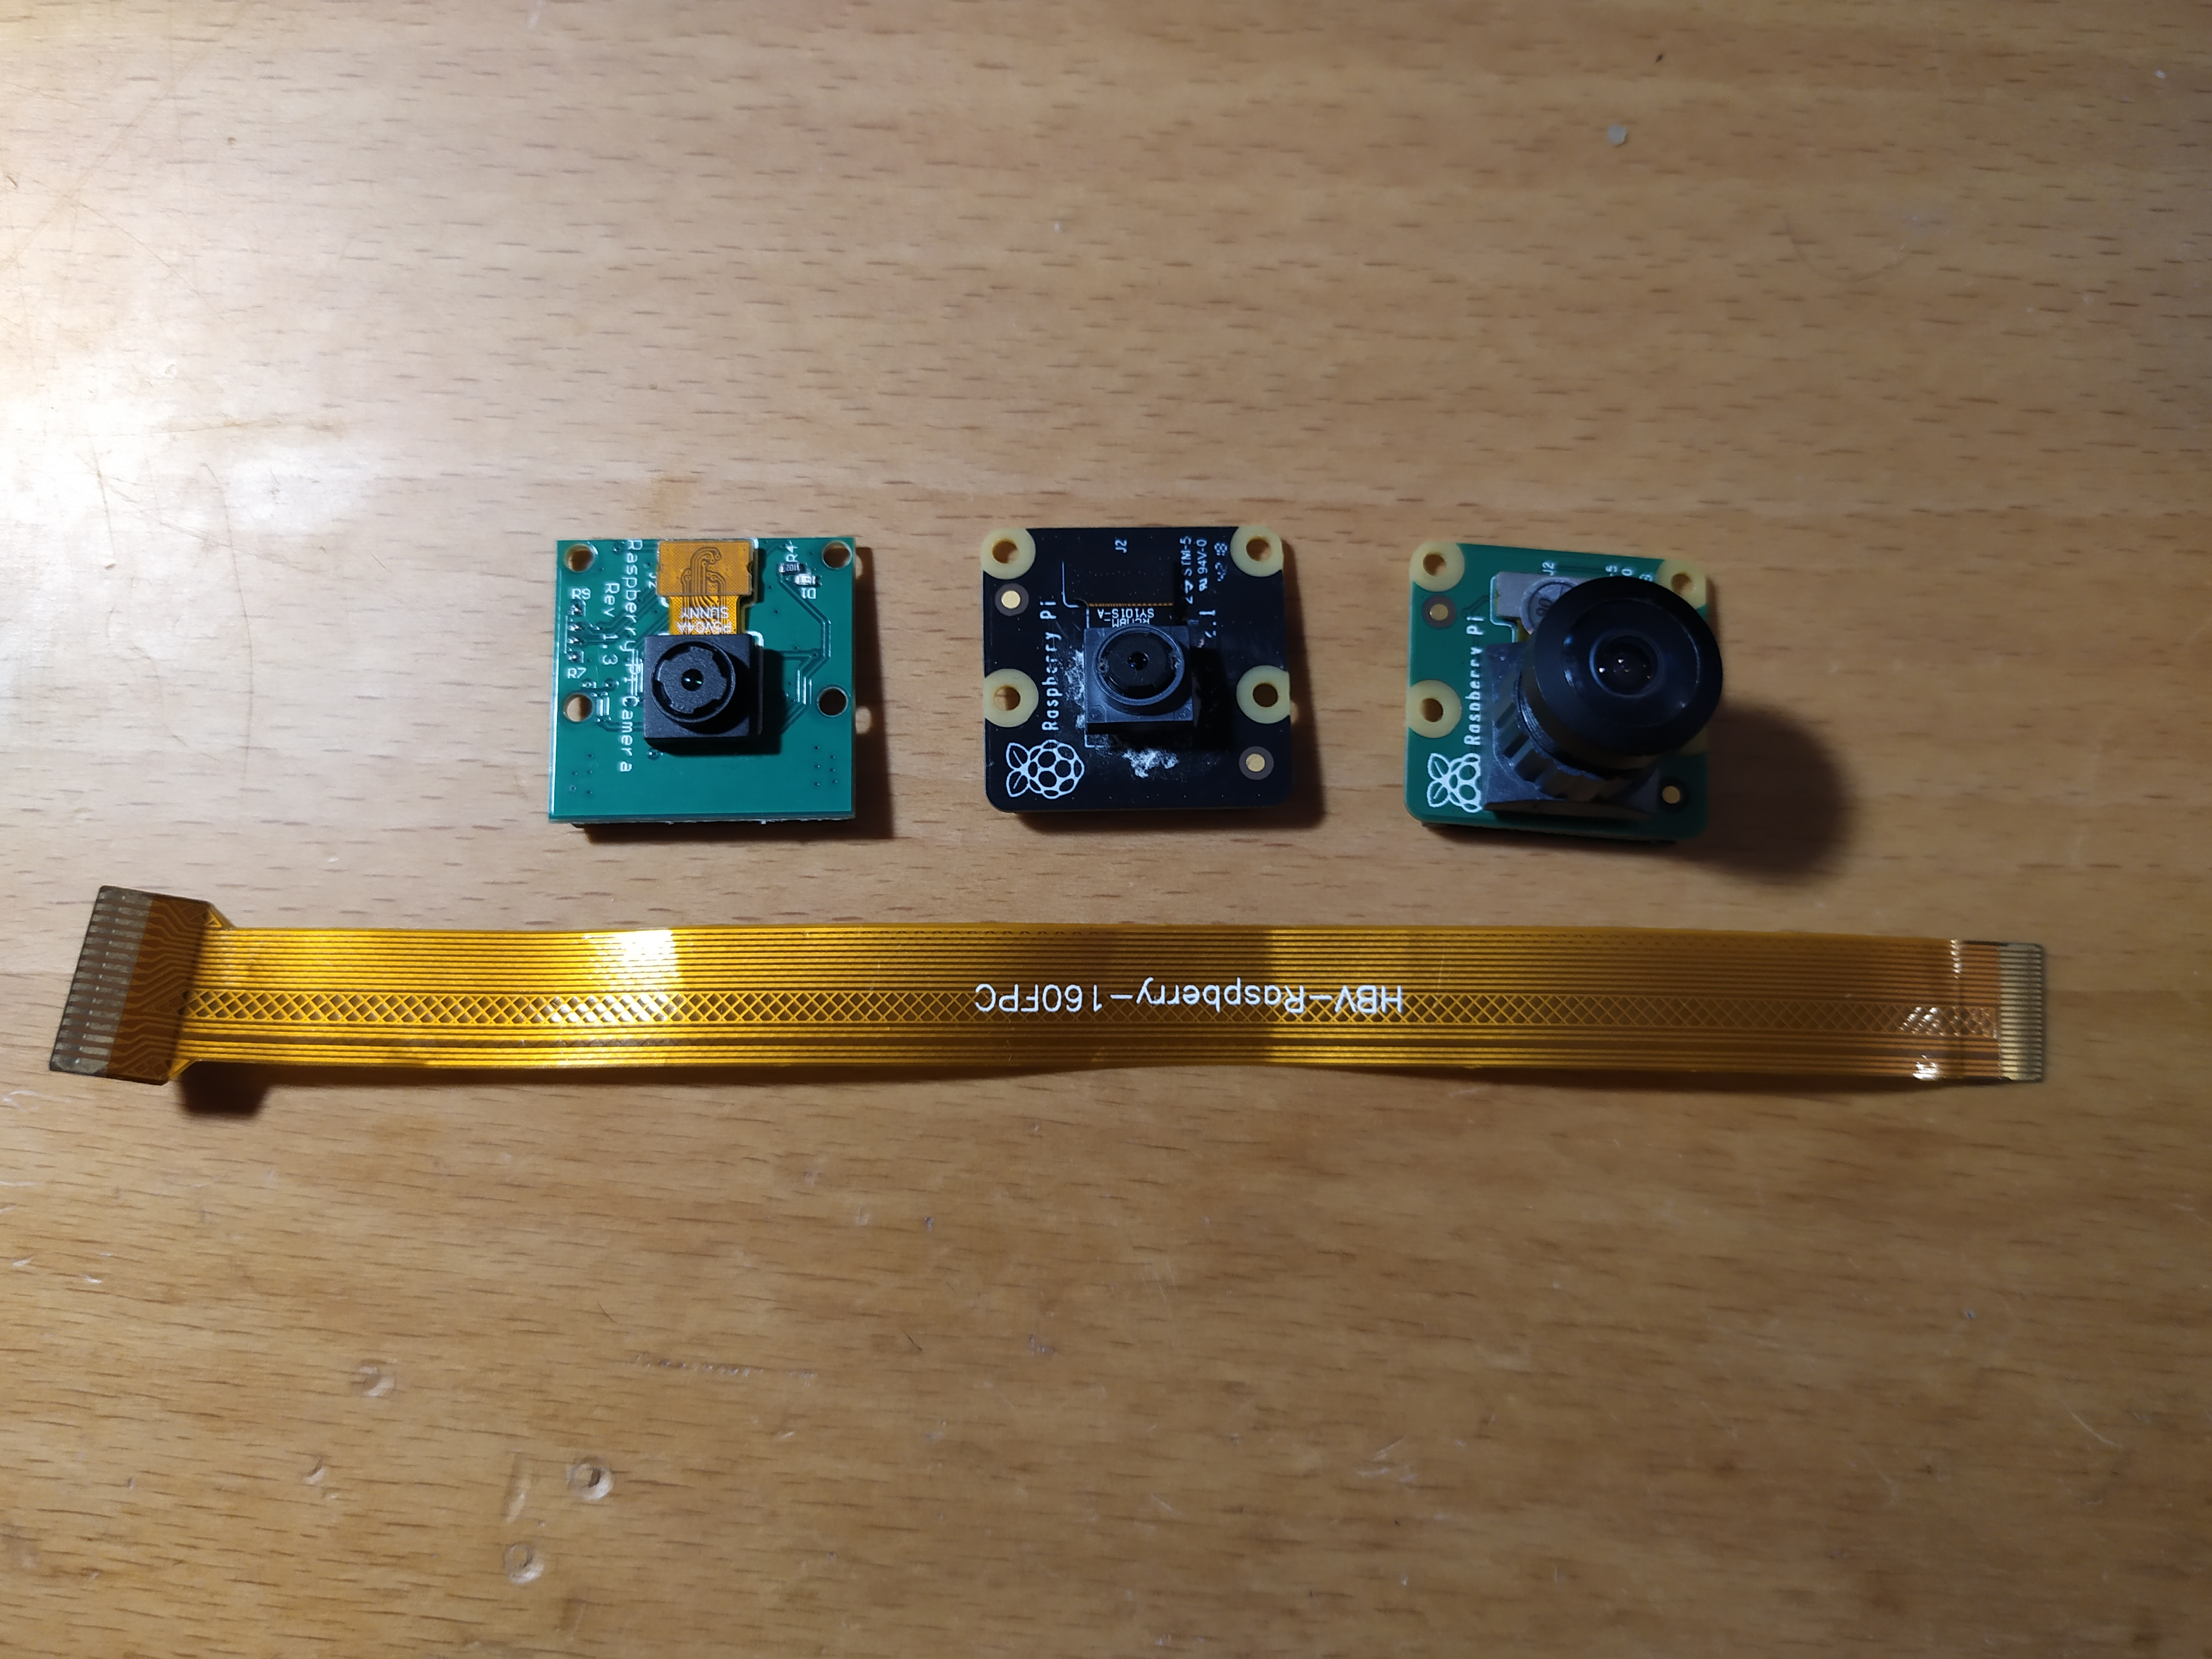
\includegraphics[scale=.06]{imaxes/camaras.jpg}
  \caption{De esquerda a dereita a Raspberry Pi camera module V1, V2 sen filtro infravermello e V2 cunha lente de gran angular}
  \label{f:Cámaras}
\end{figure}
\subsection{Lentes}
Para poder capturar o completo da estrada a cámara necesitará de algún tipo de lente que permita un maior campo de visión. Existen versións da cámara que xa inclúen unha lente, pero tamén poderemos atopar lentes externas coma es destinadas para os dispositivos móbiles, que contan co tamaño necesario para a cámara da Raspberry. Na figura 3.3 móstranse as lentes a probar e analizar as tres superiores colocaranse sobre a cámara e as tres inferiores so para a versión da cámara que incorpora lente.
\begin{figure}[tb]
  \centering
  \includegraphics[scale=.06]{imaxes/lentes.jpg}
  \caption{Lentes con diferente ángulo de visión. De esquerda a dereita: fila superior 0.67x, 180º, 0.4x, fila inferior 130º, 160º, 220º }
  \label{f:Lentes}
\end{figure}

\subsection{Captura de vídeo}
\emph{Raspivideo} é o software que utilizaremos para capturar as imaxes, o programa executase dende terminal proporcionándolle diferentes parámetros. No noso caso os parámetros a utilizar serán:
\begin{itemize}
    \item -t Tempo de captura de vídeo, no noso caso será 0 indicando que a captura será continua.
    \item -w e -h Son os parámetros de anchura e altura de píxeles, probaremos diferentes resolucións para conseguir a máxima calidade posible sempre que o tamaño da imaxe non repercuta na latencia de transmisión.
    \item -fps \emph{Frames per second}, é o numero de imaxes a capturar cada segundo, variaremos con este valor para minimizar a latencia.
    \item -b \emph{Bitrate}, o numero de bits por segundo, buscaremos o valor máis alto posible sen que produza retardos na transmisión.
    \item -n Con este parámetro deshabilitaremos a previsualización do vídeo.
    \item -pf Parámetro para elixir o perfil do codificador de vídeo H264, as opcións dispoñibles son, \emph{baseline}, \emph{main} and \emph{high}. Utilizaremos a opción \emph{baseline} xa que é a que menor custo computacional ten.
    \item -o Con este parámetro indicamos a saída de vídeo, como por exemplo a un arquivo, no noso caso utilizaremos a saída estándar que indicaremos con "-" , e que redirecionaremos máis tarde.
\end{itemize}

\section{Transmisión de vídeo}
Para transmitir o vídeo ao dispositivo móbil a través da rede preséntanse varias posibilidades. Para comparalas transmitiremos vídeo dende a Raspberry Pi cunha mesma resolución, 720p, e recibiremos e reproduciremos o nun pc mediante \emph{vlc}.

\begin{itemize}
    \item A primeira opción a analizar é o software de vídeo \emph{vlc}, unha completa ferramenta de reprodución que tamén permite a transmisión e e a recepción de vídeo na rede mediante diferentes protocolos. Faremos unha proba utilizando o \emph{vlc} na Raspberry Pi para transmitir o vídeo da cámara e recibilo nun pc con \emph{vlc}. Como resultado obtemos unha transmisión cunha latencia superior a un segundo, que imposibilita o seu uso para controlar o trafico en tempo real.

    \item A segunda opción que probaremos consistirá en capturar o vídeo coa ferramenta de captura de vídeo da Raspberry Pi, \emph{raspivid}, e redirecionar a sua saída a rede utilizando \emph{netcat} unha utilidade para transmitir e recibir na rede mediante \emph{tcp} ou \emph{udp}. Transmitiremos mediante \emph{udp} para conseguir unha menor latencia a custo de perder algún fotograma. A recepción de vídeo a realizaremos nun pc mediante \emph{vlc} coma no caso anterior. A latencia obtida neste caso e mellor que no anterior.

    \item Buscando reducir aínda máis a latencia probaremos a utilizar o software \emph{socat}, que funciona de forma similar a \emph{netcat} e conta tamén con moitas opcións de configuración. O procedemento será igual que no caso anterior, faremos a captura con \emph{raspivid} e redirecionaremos o vídeo a un porto nunha dirección \emph{ip} mediante \emph{udp} neste caso utilizando \emph{socat}. Como resultado obtemos unha latencia aínda menor que con \emph{netcat} polo que utilizaremos este software para a transmisión de vídeo.
\end{itemize}

\section{Recepción de ordes}

 Para recibir os comandos enviados dende o dispositivo móbil e executalos mediante Python implementaremos un servidor tamén Python para poder integrar a recepción e a execución de ordes no mesmo programa.

 A primeira opción será utilizar peticións \emph{http} e manexalas mediante a clase de Python \emph{BaseHTTPRequestHandler}, o problema é que esta clase bloquea o programa mentres se executan as ordes correspondentes a petición recibida. Para solucionar este problema poderiáse implementar un servidor \emph{multithread} ou utilizar unha libraría para Python que implemente o servidor \emph{multithread} de forma transparente. Plantexase utilizar as librarias \emph{multithread} \emph{Tornado}, \emph{Twisted} ou \emph{lighttpd} pero debido os recursos limitados da Rasberry Pi Zero o uso dunha destas librarías podería implicar maiores latencias e consumo enerxético.

 Finalmente optase por manexar a conexión directamente mediante \emph{sockets} non bloqueastes é así poder utilizar un solo \emph{thread}. Para elo introduciremos as peticións de conexión nunha lista, unha vez aceptada introducirase nunha segunda lista as mensaxes recibidas e se executara a orde correspondente para cada mensaxe.

As mensaxes serán as seguintes:
\begin{itemize}
    \item \textbf{r} para o xiro a dereita.
    \item \textbf{l} para o xiro a esquerda.
    \item \textbf{n} para a luz de noite.
    \item \textbf{b} para a luz de freo.
    \item \textbf{k} para o padrón de palpadeo.
    \item \textbf{o} para apagar as luces.
    \item \textbf{v} para iniciar a captura e transmisión de vídeo.
    \item \textbf{vs} para deter a captura e a transmisión de vídeo.
    \item \textbf{c} para comprobar que a conexión segue aberta.
    \item \textbf{valor numérico} para establecer a intensidade das luces.
\end{itemize}

\section{Conexión co servidor}
Os dispositivos conectaranse mediante unha rede local, xa sexa a través dun cable usb ou dunha rede wi-fi, en ámbolos dous casos o dispositivo Android será o encargado de aloxar a rede xa sexa compartindo por usb ou creando un punto de aceso wi-fi.

Para permitir que o dispositivo móbil se conecte o servidor sen ter que coñecer a dirección \emph{ip} de este procederase da seguinte maneira. Dende o servidor crearase un \emph{thread} no que se abrira un \emph{socket} encargado de enviar unha mensaxe a dirección de \emph{broadcast} para que poda ser recibido por tódolos dispositivos da rede.

\section{Autoarranque do servidor}
O servidor deberá arrancar automaticamente o acender o dispositivo, e arrancar de novo se por algún motivo detense a súa execución. Para elo crearemos un servizo en \emph{sytemd} que se encargará de arrancar o programa e reinicialo se é necesario. A estrutura do servizo e a seguinte, indica a localización do programa Python a executar, a orde de reiniciar sempre, os \emph{logs} a utilizar para rexistrar as execucións e os fallos, e o usuario e grupo que o executará. Situaremos o ficheiro do servizo na ruta \textit{/etc/systemd/system/} e unha vez ali o habilitaremos coa orde \textit{sudo systemctl enable bikeview.service} agora o servizo executarase cando se arranque o dispositivo e reiniciarase se se para.

\section{Alimentación e enerxía}
O consumo de amperios da Raspberry Pi Zero sen carga de traballo é duns 120 mA, gravando vídeo a 1080p o consumo é de 230mA, gravarase vídeo a 720p polo que o consumo será algo menor pero engadirase o consumo do chip wifi funcionando. Os leds ws2812 teñen un consumo máximo de 60 mA cada un 20 mA como máximo por cada un dos tres leds \emph{RGB} a máxima intensidade, o noso máximo consumo realizarse coa luz vermella acesa de forma continua, xa que no resto de modos os padróns de palpadeo reducen o consumo. Contamos con 24 destes leds polo que o consumo máximo será de 20mA por 24 leds, un total de 480mA que sumados o consumo da Raspberry Pi nos da un consumo máximo teórico de 710mA na versión sen leds intermitentes o consumo seria de 160mA máis 230mA, en total 390mA.

\begin{itemize}
    \item Unha primeira versión máis sinxela contará solo cunha batería usb para alimentar a Raspberry. Os requisitos de esta batería serán a amperaxe e a capacidade.

    Partirase do valor do consumo máximo aproximado de 400mA para calcular o tempo de funcionamento. Con esta amperaxe aos 5V que funcionan a Raspberry e os leds a potencia utilizada sería de 2W. Neste suposto unha batería de  5000mAh cunha voltaxe nominal de 3.7V pode proporcionar 18.5Wh polo que duraría ata 9 horas e 15 minutos, no caso dunha batería de 1000mAh o tempo mínimo teórico de funcionamento sería de algo menos de dúas horas.
    Comprobaremos se estes supostos se cumpren facendo medicións do tempo de funcionamento.

    \item Realizaremos unha segunda versión máis avanzada que apagará o dispositivo cando a batería baixe de certo limite de voltaxe para evitar que o dispositivo se desconecte e contará tamén cun pulsador para poder acendela e apagala.

    Para isto utilizaremos o chip de carga Adafruit Powerboost 1000 que conta cunhas características moi interesantes a maiores da protección de sobrecarga conta cunha led e un pin que se activaran cando a voltaxe da batería baixe dos 3.2v, unha voltaxe operacional de 5.2v para evitar perdidas de voltaxe en cables e conectores, un pin habilitador que permite conectar ou desconectar a batería, e proporciona 1 amperio de intensidade sen baixar a voltaxe dos 5v. Non conta con protección de sobrecarga polo que as batería que utilicemos deben incluír un circuíto de protección, este é o caso da maioría de baterías, de utilizar unha sin protección, como unha cela 18650, deberemos engadir o circuíto de protección ou asegurarnos de implementar o apagado por voltaxe baixa correctamente.

    A realización o circuíto basearase no guía \emph{lipopi} de Daniel Bull que utiliza o Adafruit Powerboost, nas súas dúas versións a de 500 mA e 1 A, para programar o apagado automático da Rapberry Pi cando a batería baixe de 3.2v e un pulsador para o acendido, tamén conta con dúas versións máis unha que tamén permite o apagado, e outra que monitoriza a voltaxe da batería. Realizarase a versión con pulsador para acendido e apagado.

    O funcionamento é o seguinte, o premer o pulsador conéctase o positivo da batería co pin abilitador, acendendo o adafruit powerboost e por conseguinte acendendo a Raspberry Pi. O acender a Raspberry Pi un pin conectado o pin habilitador acenderase pare seguir mantendo un valor positivo. Para evitar que o voltaxe no pin habilitador caia no tempo entre que pulsamos o pulsador e a Raspberry Pi arranca e encárgase de manter o valor positivo, situaremos un circuíto RC formado por un condensador cunha resistencia en paralelo entre o pulsador e o pin habilitador. O condensador cargarase cando o pulsador cerre o circuíto e descargarase a continuación mantendo a voltaxe o tempo suficiente para que a Raspberry arranque e acenda o pin. Utilizarase un condensador de 100\(\mu\)F xunto cunha resistencia 100k\(\Omega\) que proporcionan un tempo suficiente de 10 segundos. O pin da Raspberry que utilizaremos para este propósito pode ser o 14 correspondente a conexión \emph{uart}, que se acenderá coa Raspberry e se desconectará cando se apague, engadiremos unha resistencia de 10k\(\Omega\) para protexer este pin. Tamén poderíase utilizar calquera outro pin de propósito xeral indicando no arquivo de configuración \emph{config.txt} na partición \emph{boot} da Raspberry, que o pin arranque cun valor positivo e cun valor negativo cando o dispositivo se apague, no caso de utilizar o pin \emph{GPIO} 5 as ordes serían as seguintes: \emph{$gpio=5=op,dh$} para que o pin arranque con valor positivo, \emph{$dtoverlay=gpio-poweroff,gpiopin=5,active_low="y"$} para deixar o pin apagado cando se apaga a Raspberry.

    Para o apagado utilizarase un segundo pin conectado o pulsador, cando este se pulse, estando a Rasberry acesa, se conectará a voltaxe da batería, cando este valor positivo chegue o pin un script Python encargarase de apagar o dispositivo. Engadiranse un divisor de voltaxe para reducir a voltaxe da batería xa que cando está completamente cargada a sua voltaxe de 4.2v e superior o máximo valor lóxico tolerado pola Raspberry Pi de 3.3V. Utilizaremos unha resistencia de 33k\(\Omega\) conectada entre o pin e a batería e unha resistencia de 100k\(\Omega\) entre o pin e terra. Para evitar que o pin de acendido dispare o apagado situarase un díodo entre o pin de acendido e apagado evitando que a voltaxe circule nesa dirección.

    Finalmente conectarase o pin indicador de batería baixa a outro pin de entrada da Raspberry que mediante o script Python apagará o dispositivo. O diagrama de funcionamento mostrase na figura 3.4.

    \begin{figure}[tb]
      \centering
    	\includegraphics[scale=1]{imaxes/circuito-bateria.png}
    	\caption{Diagrama de funcionamento do circuíto de alimentación.}
    	\label{f:circuíto de alimentación}
    \end{figure}

    Na figura 3.5 podemos ver o diagrama final do dispositivo e na figura 3.6 o esquema completo integrando os leds o circuíto de carga e a cámara.

    \begin{figure}[tb]
      \centering
    	\includegraphics[scale=1]{imaxes/circuito-completo.png}
    	\caption{Diagrama do dispositivo.}
    	\label{f:circuíto do dispositivo}
    \end{figure}

    \begin{sidewaysfigure}[tb]
      \centering
    	\includegraphics[scale=1]{imaxes/esquema-completo.png}
    	\caption{Esquema completo do dispositivo.}
    	\label{f:esquema do dispositivo}
    \end{sidewaysfigure}

    Para arrancar automaticamente o script Python instalarase un novo servizo en \emph{sytemd} e de igual maneira que co servidor executarase no arranque e cada vez que se pare.

    Na implementación física colocaremos o chip de carga xunto cos compoñentes electrónicos nunha placa cun conector para poder conectalo directamente os conectores da Raspberry Pi Zero. Tamén colocarase nesta placa o conversor lóxico de nivel como se ve na figura

    \begin{figure}[tb]
      \centering
    	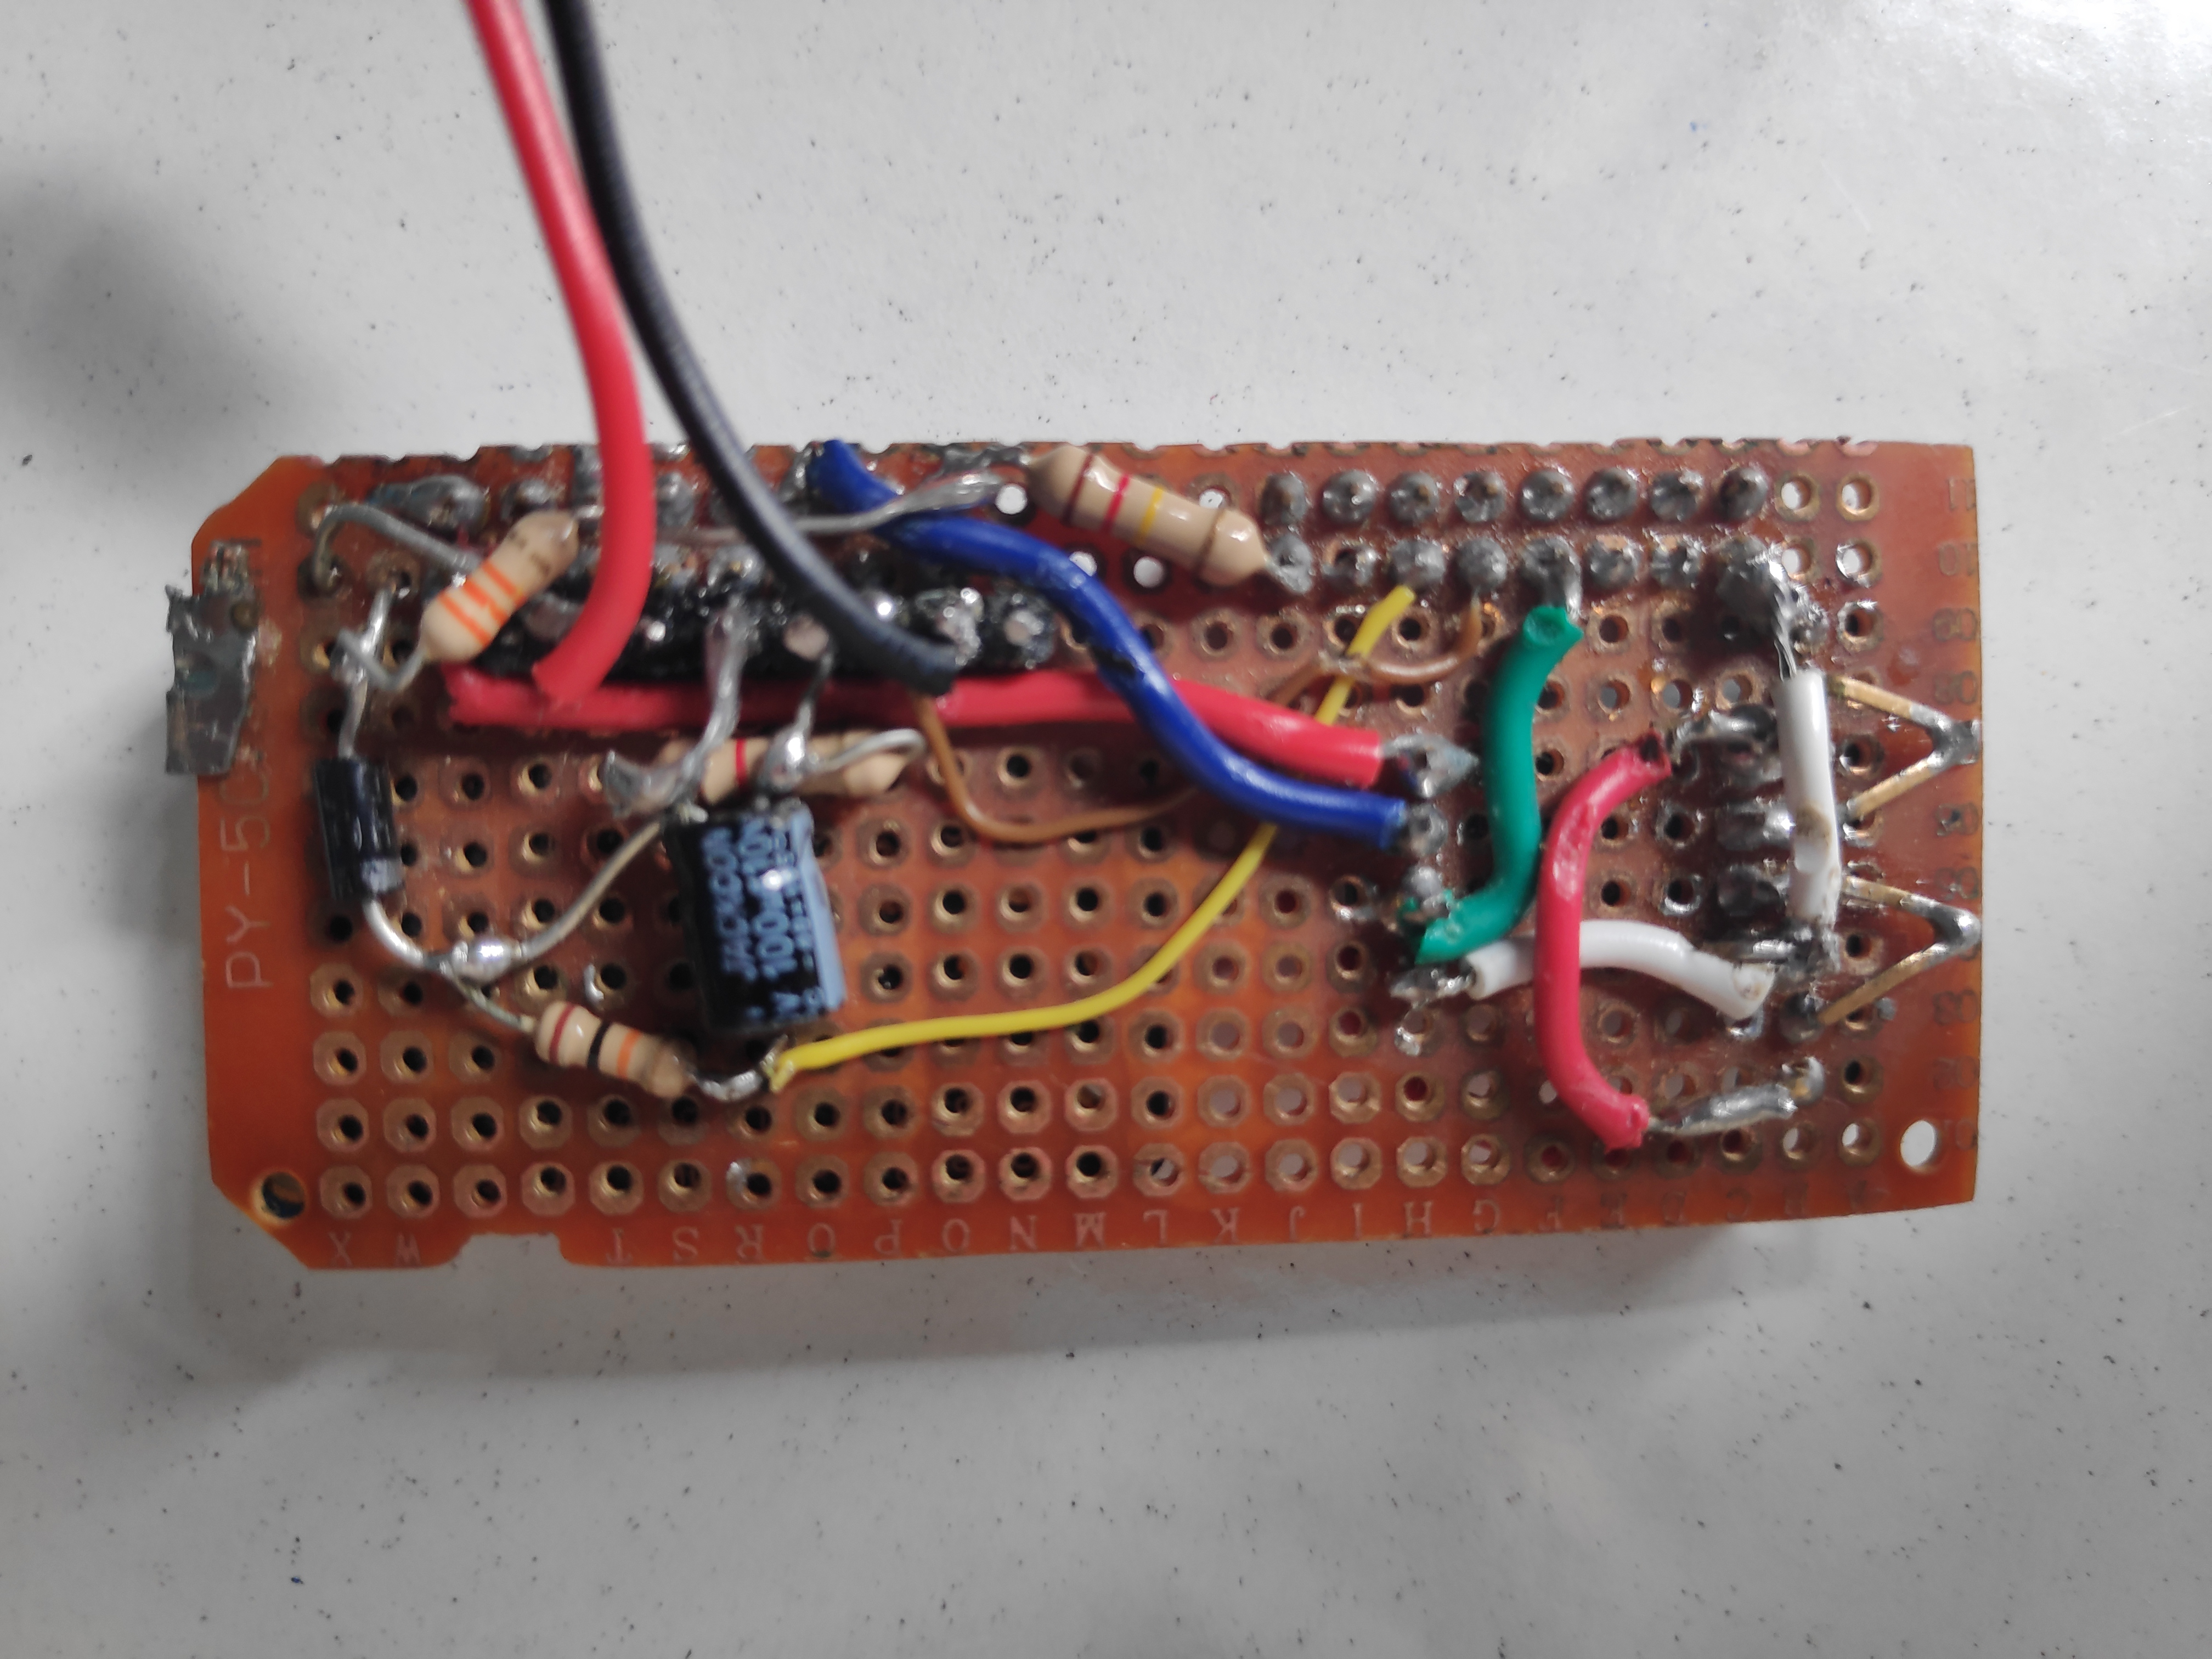
\includegraphics[scale=.05]{imaxes/foto-circuito1.jpg}
    	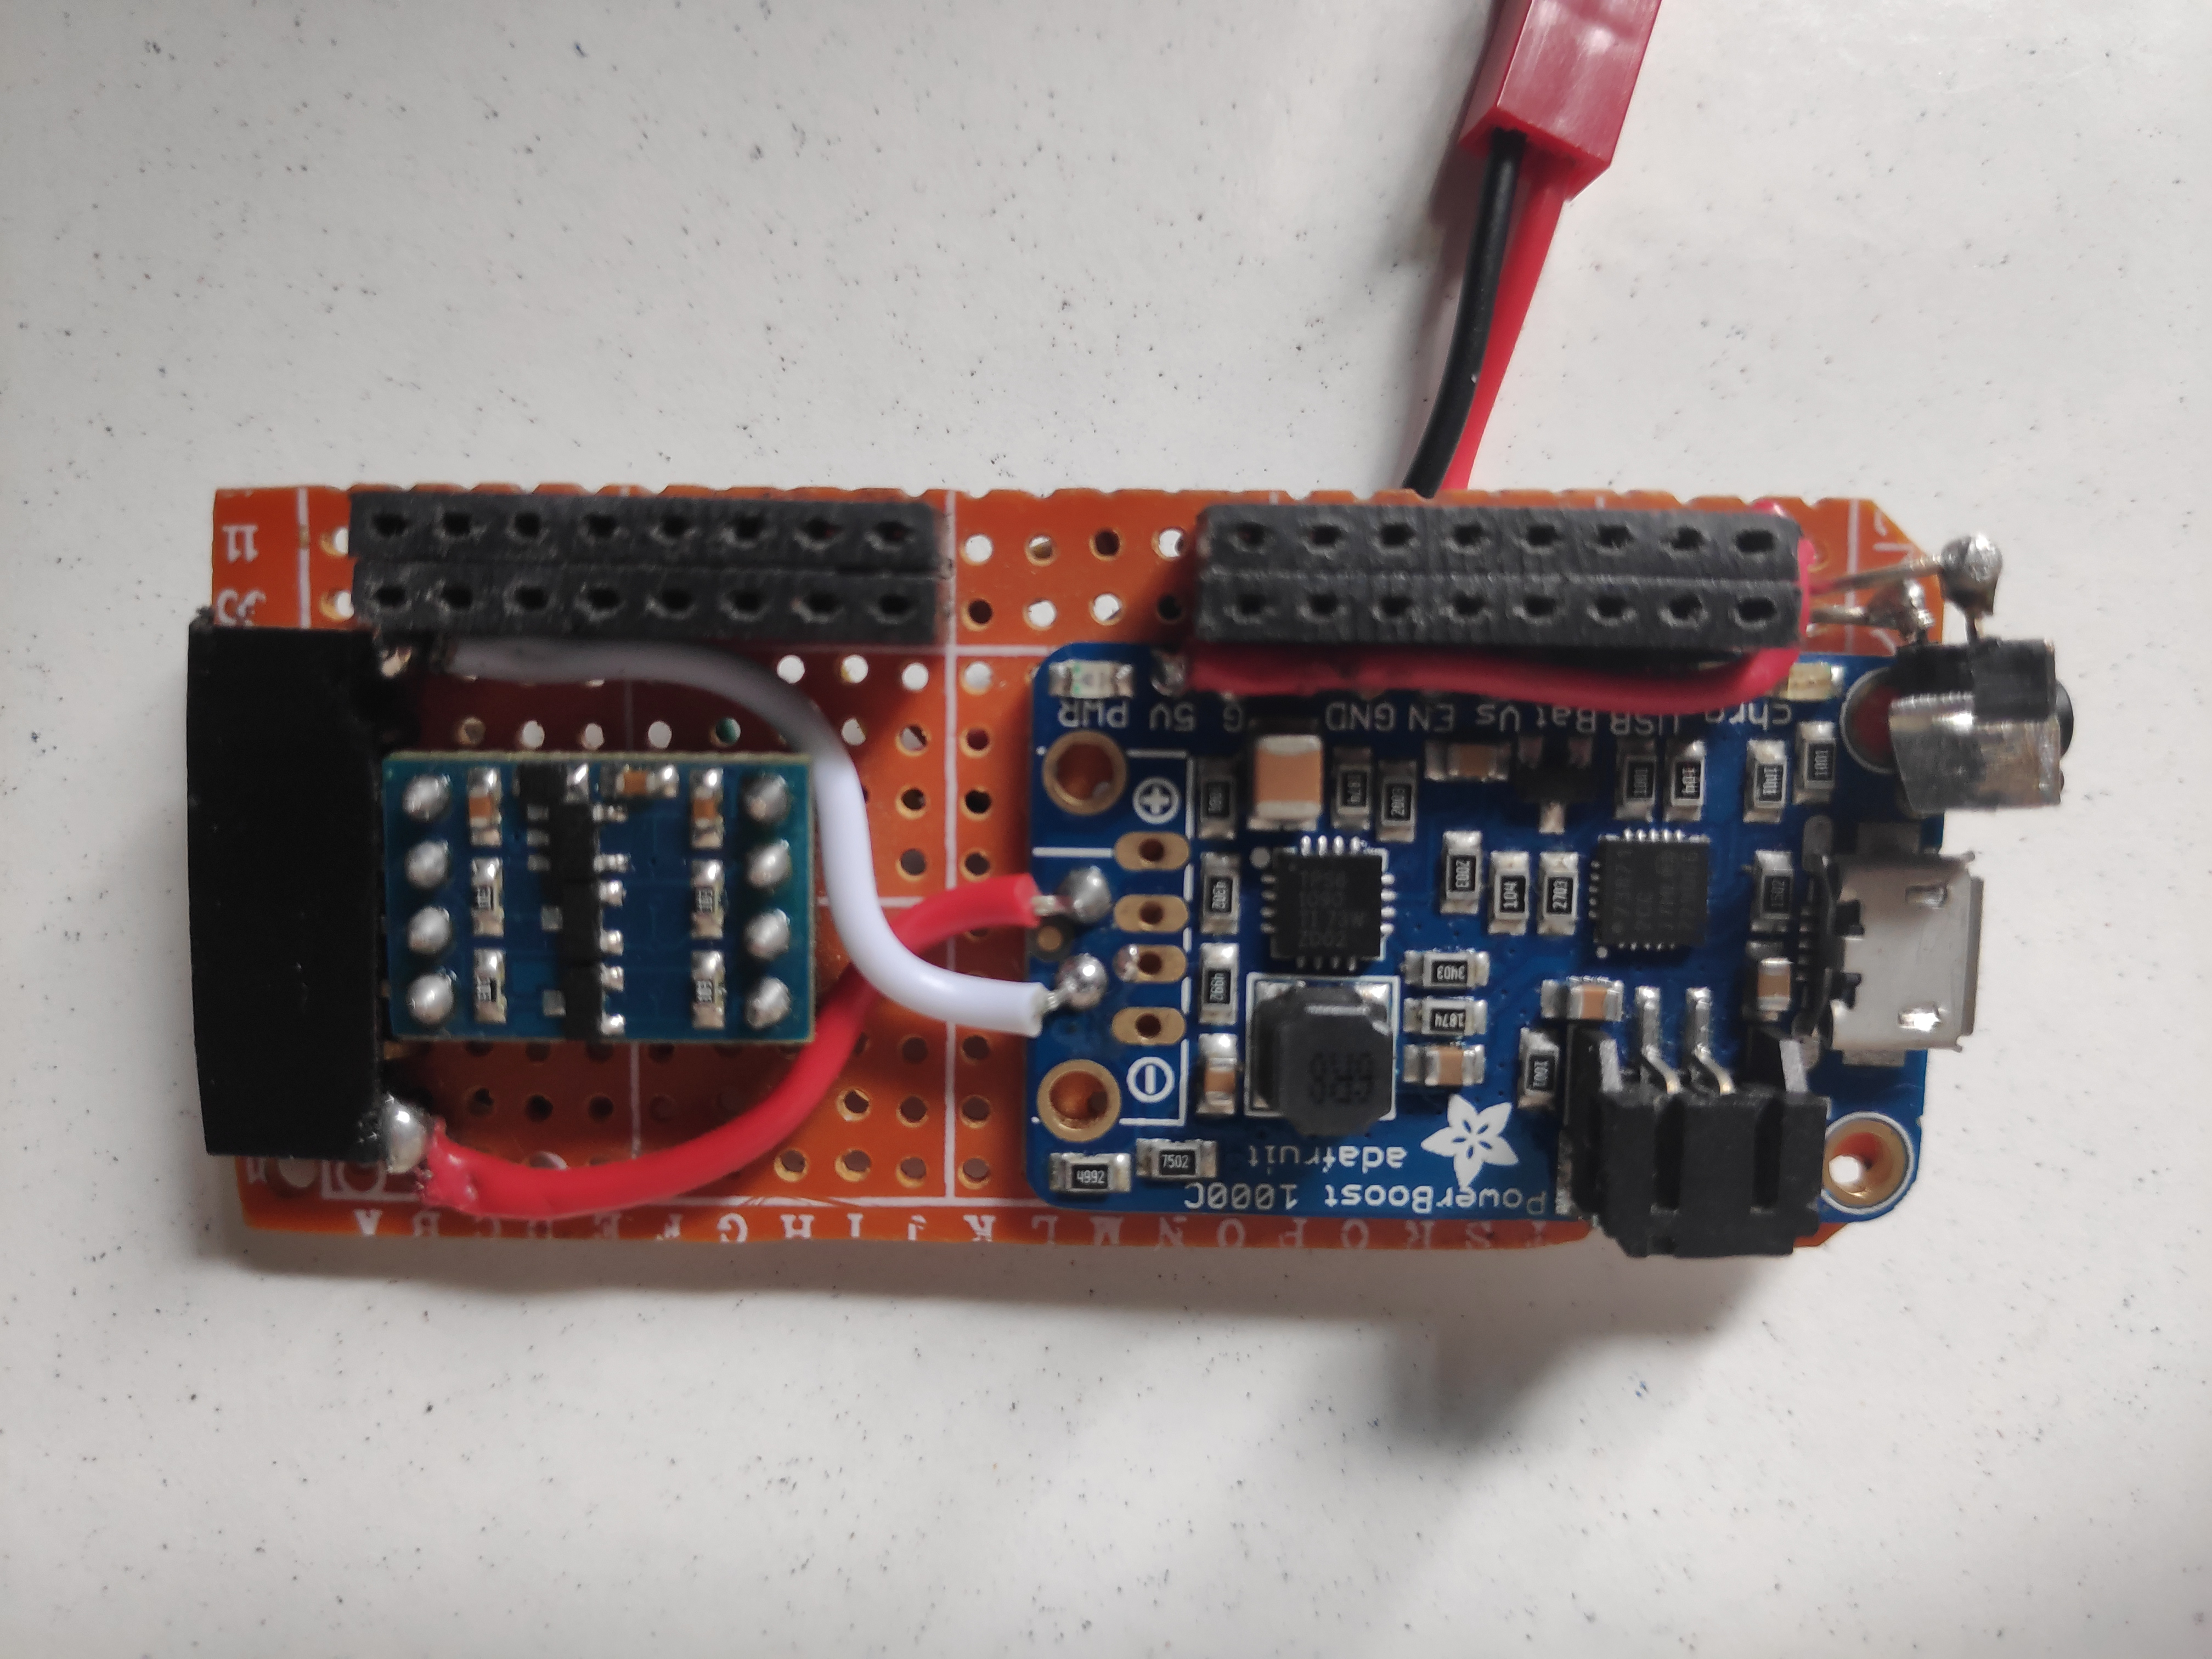
\includegraphics[scale=.05]{imaxes/foto-circuito2.jpg}
    	\caption{Imaxes do circuíto por ambas caras.}
    	\label{f:fotos do circuíto reverso}
    \end{figure}

    Na elección da batería teremos en conta a maiores da sua capacidade o seu tamaño e forma, sendo o ideal que sexa similar o da Raspberry para poder integrala no dispositivo con facilidade. Por eso elixiremos unha batería de 1600mA e 5.92Wh con circuíto de protección e unhas dimensións de 9 x 34 x 50mm que para este suposto, xa que engadindo os leds extra calcúlase un consumo máximo de 3.55W, debería proporcionar un tempo mínimo de funcionamento de 2 horas aproximadamente.

\end{itemize}

\section{Carcasa e ancoraxe}

Para protexer o dispositivo e suxeitalo baixo a sela da bicicleta plantexaranse dúas opcións.
\begin{itemize}
    \item A primeira realizarase para a versión do proxecto alimentada cunha batería usb. Consistirá en utilizar a carcasa oficial da Raspberry Pi Zero que inclúe un oco para a cámara e espazo para as conexión na parte de atrás, a carcasa so permite a uso de cámaras sen lentes polo que incorporarase unha lente externa.

    Para suxeitar a carcasa a bicicleta deseñaremos un soporte en 3d co software Blender. Partiremos das medición da carcasa e deseñarase un soporte que suxeite a carcasa firmemente e permita atala a barra da sela mediante unha correa.

    Unha vez deseñado e tras comprobar que o deseño e imprimible exportarase no formato \emph{STL} que abrirase cun software encargado de dividir o deseño en capas e traducilo a ordes de desprazamento interpretables pola impresora, aquí configuraranse diferentes parámetros como a altura de capa, que é a resolución de impresión, as velocidades, a cantidade e tipo de recheo da peza ou o uso de soportes para facilitar a impresión. Neste caso utilizaras o software libre Slic3r no que configurarase a peza a imprimir cun 100\(\%\) de recheo para que sexa máis sólida cunha altura de capa de 0.2mm e sen uso de soportes, como resultado obterase un arquivo \emph{GCODE}  que pasaremos a impresora. O prototipo imprimirase o prototipo en 3d probarase e aplicaranse correccións no modelo. Para este deseño realizáronse dúas iteracións móstranse na figura 3.6.

    \begin{figure}[tb]
      \centering
      \includegraphics[scale=.1]{imaxes/soporte-caixa.jpg}
      \caption{Deseños do soporte.}
      \label{f:soporte caixa}
    \end{figure}


    \item A segunda versión terá que albergar a Raspberry Pi Zero xunto coa cámara, o chip de carga e alimentación, o conversor lóxico de voltaxe e a batería. Utilizaremos tamén neste caso o software de edición 3d Blender para deseñar os prototipos.

    O deseño contara co anel led situado no exterior o redor da lente da cámara, no interior colocaranse tódolos compoñentes electrónicas e a batería. Na parte superior contará cun oco para o conector micro usb de carga e aceso a tarxeta micro sd da Raspberry Pi. No exterior contará tamén con dous brazos articulados nos que situaremos as dúas tiras leds para indicar o xiro.

    Da mesma forma que no caso anterior o deseño imprimirase modificarase e volverase a imprimir ata que se obteña un resultado aceptable. Na figura 3.7 pódese observar a evolución dos diferentes deseños e na figura 3.8 unha imaxe renderizada do deseño final.


    \begin{figure}[tb]
      \centering
      \includegraphics[scale=.1]{imaxes/evolucion-carcasa.jpg}
      \caption{Evolución dos deseños da carcasa.}
      \label{f:evolucion da carcasa}
    \end{figure}

    \begin{figure}[tb]
      \centering
      \includegraphics[scale=.4]{imaxes/carcasa.png}
      \caption{Ultimo desño da carcasa.}
      \label{f:carcasa}
    \end{figure}

    \section{Custo do dispositivo}
    Para aproximar o rango prezos do custo de fabricación do dispositivo calcularanse dúas opción a primeira utilizando os compoñentes máis baratos é a segunda os máis caros.
    \begin{table}[tb]
        \label{c:custos dispositivo}
        \begin{center}
            \begin{tabular}{|l|l||l|l|}
                \hline
                 Menor prezo & Custo  & Maior Prezo & Custo \\ \hline
                 Raspberry Pi Zero & 5.00€  & Raspberry Pi Zero W& 11.00€ \\ \hline
                 Adaptador Wi-Fi usb & 1.00€ &  & \\ \hline
                 Carcasa 3D & 0.50€ & Carcasa ofical & 6.00€ \\ \hline
                  &  & Soprte 3D & 0.50€ \\ \hline
                 Pi Camera Module V1 & 3.00€ & Pi Camera Module V2 & 20.00€ \\ \hline
                  &  & Lentes  & 2.00€ \\ \hline
                 8 leds w2812b & 1.00€  &  24 leds w2812b & 3.00€\\ \hline
                 Circuito de carga e protección xenérico & 2.00€  & Adafruit Powerboost 1000C & 23.00€ \\ \hline
                 Batería Lipo 1600mA & 7.00€ & Batería Lipo 1800mA & 10.00€\\ \hline
                 Cables & 1.00€ &  Cables & 1.00€ \\ \hline
                 Total & 20.50€ &  Total & 76.50€ \\ \hline
            \end{tabular}
        \end{center}
        \caption{Custos monetarios do proxecto}
    \end{table}
\end{itemize}
